\documentclass[12pt, spanish]{article}

\usepackage{graphicx}
\usepackage[a4paper, total={6in, 9in}]{geometry}
\usepackage[spanish]{babel}
\usepackage{translator}
\usepackage{titlesec}
\usepackage{pgfgantt}
\usepackage{url}
\usepackage{longtable}
\usepackage{booktabs}
\usepackage{siunitx}
\usepackage{float}
\usepackage{fancyvrb}
\usepackage[normalem]{ulem}
\usepackage{listings}
\usepackage{subfig}
\usepackage{pdflscape}

% PANDOC


\usepackage{lmodern}
\usepackage{amssymb,amsmath}
\usepackage{ifxetex,ifluatex}
\ifnum 0\ifxetex 1\fi\ifluatex 1\fi=0 % if pdftex
\usepackage[T1]{fontenc}
\usepackage[utf8]{inputenc}
\usepackage{textcomp} % provide euro and other symbols
\else % if luatex or xetex
\usepackage{unicode-math}
\defaultfontfeatures{Scale=MatchLowercase}
\defaultfontfeatures[\rmfamily]{Ligatures=TeX,Scale=1}
\fi
% Use upquote if available, for straight quotes in verbatim environments
\IfFileExists{upquote.sty}{\usepackage{upquote}}{}
\IfFileExists{microtype.sty}{% use microtype if available
	\usepackage[]{microtype}
	\UseMicrotypeSet[protrusion]{basicmath} % disable protrusion for tt fonts
}{}
\makeatletter
\@ifundefined{KOMAClassName}{% if non-KOMA class
	\IfFileExists{parskip.sty}{%
		\usepackage{parskip}
	}{% else
		\setlength{\parindent}{0pt}
		\setlength{\parskip}{6pt plus 2pt minus 1pt}}
}{% if KOMA class
	\KOMAoptions{parskip=half}}
\makeatother
\usepackage{xcolor}
\IfFileExists{xurl.sty}{\usepackage{xurl}}{} % add URL line breaks if available
\IfFileExists{bookmark.sty}{\usepackage{bookmark}}{\usepackage{hyperref}}
\urlstyle{same} % disable monospaced font for URLs
\hypersetup{%
hidelinks = true
}
\usepackage{color}
\usepackage{fancyvrb}
\newcommand{\VerbBar}{|}
\newcommand{\VERB}{\Verb[commandchars=\\\{\}]}
\DefineVerbatimEnvironment{Highlighting}{Verbatim}{commandchars=\\\{\}}
% Add ',fontsize=\small' for more characters per line
\newenvironment{Shaded}{}{}
\newcommand{\AlertTok}[1]{\textcolor[rgb]{1.00,0.00,0.00}{\textbf{#1}}}
\newcommand{\AnnotationTok}[1]{\textcolor[rgb]{0.38,0.63,0.69}{\textbf{\textit{#1}}}}
\newcommand{\AttributeTok}[1]{\textcolor[rgb]{0.49,0.56,0.16}{#1}}
\newcommand{\BaseNTok}[1]{\textcolor[rgb]{0.25,0.63,0.44}{#1}}
\newcommand{\BuiltInTok}[1]{#1}
\newcommand{\CharTok}[1]{\textcolor[rgb]{0.25,0.44,0.63}{#1}}
\newcommand{\CommentTok}[1]{\textcolor[rgb]{0.38,0.63,0.69}{\textit{#1}}}
\newcommand{\CommentVarTok}[1]{\textcolor[rgb]{0.38,0.63,0.69}{\textbf{\textit{#1}}}}
\newcommand{\ConstantTok}[1]{\textcolor[rgb]{0.53,0.00,0.00}{#1}}
\newcommand{\ControlFlowTok}[1]{\textcolor[rgb]{0.00,0.44,0.13}{\textbf{#1}}}
\newcommand{\DataTypeTok}[1]{\textcolor[rgb]{0.56,0.13,0.00}{#1}}
\newcommand{\DecValTok}[1]{\textcolor[rgb]{0.25,0.63,0.44}{#1}}
\newcommand{\DocumentationTok}[1]{\textcolor[rgb]{0.73,0.13,0.13}{\textit{#1}}}
\newcommand{\ErrorTok}[1]{\textcolor[rgb]{1.00,0.00,0.00}{\textbf{#1}}}
\newcommand{\ExtensionTok}[1]{#1}
\newcommand{\FloatTok}[1]{\textcolor[rgb]{0.25,0.63,0.44}{#1}}
\newcommand{\FunctionTok}[1]{\textcolor[rgb]{0.02,0.16,0.49}{#1}}
\newcommand{\ImportTok}[1]{#1}
\newcommand{\InformationTok}[1]{\textcolor[rgb]{0.38,0.63,0.69}{\textbf{\textit{#1}}}}
\newcommand{\KeywordTok}[1]{\textcolor[rgb]{0.00,0.44,0.13}{\textbf{#1}}}
\newcommand{\NormalTok}[1]{#1}
\newcommand{\OperatorTok}[1]{\textcolor[rgb]{0.40,0.40,0.40}{#1}}
\newcommand{\OtherTok}[1]{\textcolor[rgb]{0.00,0.44,0.13}{#1}}
\newcommand{\PreprocessorTok}[1]{\textcolor[rgb]{0.74,0.48,0.00}{#1}}
\newcommand{\RegionMarkerTok}[1]{#1}
\newcommand{\SpecialCharTok}[1]{\textcolor[rgb]{0.25,0.44,0.63}{#1}}
\newcommand{\SpecialStringTok}[1]{\textcolor[rgb]{0.73,0.40,0.53}{#1}}
\newcommand{\StringTok}[1]{\textcolor[rgb]{0.25,0.44,0.63}{#1}}
\newcommand{\VariableTok}[1]{\textcolor[rgb]{0.10,0.09,0.49}{#1}}
\newcommand{\VerbatimStringTok}[1]{\textcolor[rgb]{0.25,0.44,0.63}{#1}}
\newcommand{\WarningTok}[1]{\textcolor[rgb]{0.38,0.63,0.69}{\textbf{\textit{#1}}}}
\usepackage{graphicx}
\makeatletter
\def\maxwidth{\ifdim\Gin@nat@width>\linewidth\linewidth\else\Gin@nat@width\fi}
\def\maxheight{\ifdim\Gin@nat@height>\textheight\textheight\else\Gin@nat@height\fi}
\makeatother
% Scale images if necessary, so that they will not overflow the page
% margins by default, and it is still possible to overwrite the defaults
% using explicit options in \includegraphics[width, height, ...]{}
\setkeys{Gin}{width=\maxwidth,height=\maxheight,keepaspectratio}
% Set default figure placement to htbp
\makeatletter
\def\fps@figure{htbp}
\makeatother
\setlength{\emergencystretch}{3em} % prevent overfull lines
\providecommand{\tightlist}{%
	\setlength{\itemsep}{0pt}\setlength{\parskip}{0pt}}

% END PANDOC

\titleformat{\chapter}[block]
{\normalfont\huge\bfseries}{\thechapter.}{1em}{\Huge}
\titlespacing*{\chapter}{0pt}{-19pt}{0pt}

\begin{document}
	
	\begin{titlepage}
		\title{
			\Huge Repast for High Performance Computing\\ Informe\\
			\vspace{20pt}
			\Large{Sistemas de Tiempo Real $|$ Ingeniería en Computación}
		}
		
		\author{
			\vspace{20pt}\\
			Arreche, Cristian\\
			Paradiso, Martín
		}
		
		\date{\today}
		
		\begin{figure}[b]
		\centering
		\Large{Facultad de Informática}\\
		\vspace{2pt}
		\Large{Universidad Nacional de La Plata}\\
		\vspace{10pt}
		
\includegraphics[width=0.2\linewidth]{logo_unlp.jpg}

		\end{figure}
	
	\maketitle
	\end{titlepage}
	\thispagestyle{empty}
	
	\tableofcontents
	
	% 1
	\section{Introducción}

\subsection{Repast HPC}

Repast for High Performance Computing es un framework de C++ orientado a
simulación y modelado paralelo basado en agentes. Implementa los mismos
conceptos que Repast Symphony, pero llevado a cómputo distribuido
paralelo de alto rendimiento.

\subsection{Alcance de este informe}

Este informe tiene como objetivo dar una reseña general del framework y
obtener métricas sencillas sobre su rendimiento, profundizando en
ciertos áspectos técnicos que suelen ser errores comunes a la hora de
utilizar la herramienta.

	\section{Análisis de Repast for High Performance Computing}

\subsection{Análisis General}

Repast HPC es una herramienta para el desarrollo de simulaciones y
modelados basados en agentes escrito en C++. Está completamente
orientado al procesamiento paralelo, para esto se apoya en alguna
implementación de MPI (``Message Passing Interface'') y un wrapper
provisto por la librería Boost.

Al ser un framework brinda toda la estructura para desarrollar la
simulación y el modelado. De manera resumida, posee las siguientes
características:

\begin{itemize}
	\tightlist
	\item
	Jerarquía de clases que imitan los objetos de LOGO; Turtles, Patches,
	Links y Observer.
	\item
	Schedulling de eventos, que permite programar eventos periódicos, y
	tener algo similar al paso del tiempo.
	\item
	Contextos, lugar donde residen los agentes.
	\item
	Proyecciones espaciales y lógicas, permiten establecer relaciones
	entre agentes.
	\item
	Comunicación entre procesos, dado las características paralelas del
	framework.
\end{itemize}

Puede utilizarse en cualquier sistema *nix, incluyendo MacOS, Linux y
FreeBSD.

\subsection{Compilación}

Al estar desarrollado en C++, que carece de un gestor de paquetes como
otros lenguajes, las dependencias se tornan problemáticas. Debido a
esto, Repast provee un archivo con las librerías y versiones apropiadas:

\url{https://github.com/Repast/repast.hpc/releases/tag/v2.3.0}

Las librerías de las que depende Repast son:

\begin{itemize}
	\tightlist
	\item
	Herramientas de compilación (g++, make, diff).
	\item
	MPI
	\item
	NetCDF
	\item
	CURL
	\item
	Boost: serialization, system, filesystem y mpi.
\end{itemize}

\subsubsection{Instalación de Dependencias}

La manera más efectiva de instalar todas las dependencias es utilizar el
archivo mencionado anteriormente, siguiendo las instrucciones para la
instalación manual, para el caso de un Linux basado en Debian, los
comandos a ejecutar son los siguientes:

\begin{Shaded}
	\begin{Highlighting}[]
		\BuiltInTok{cd}\NormalTok{ MANUAL\_INSTALL}
		
		\ExtensionTok{apt{-}get}\NormalTok{ update }\KeywordTok{\&\&} \ExtensionTok{apt{-}get}\NormalTok{ install build{-}essential}
		
		\ExtensionTok{./install.sh}\NormalTok{ curl}
		\ExtensionTok{./install.sh}\NormalTok{ mpich }
		\BuiltInTok{export} \VariableTok{PATH=$HOME}\NormalTok{/sfw/MPICH/bin/:}\VariableTok{$PATH}
		\ExtensionTok{./install.sh}\NormalTok{ netcdf}
		\ExtensionTok{./install.sh}\NormalTok{ boost}
		\ExtensionTok{./install.sh}\NormalTok{ rhpc}
	\end{Highlighting}
\end{Shaded}

Todas las librerías y headers son instalados en la carpeta
\texttt{\textasciitilde{}/sfw/}. En la línea 7 se agrega la carpeta de
MPICH a la variable PATH para que Boost y la terminal puedan encontrar
el binario de MPI.

Para ver ejemplos de compilación, puede usarse como guía los ejemplos
que se encuentran en:
\url{https://repast.github.io/hpc_tutorial/TOC.html}.

\subsection{Ejecución}

El binario generado debe ejecutarse a través de MPICH (u otra
implementación de MPI), para que se genere el entorno adecuado,
especificando la cantidad de procesos:

\begin{verbatim}
mpirun -n P repast.exe
\end{verbatim}

Siendo P la cantidad de procesos, también puede enviarse parámetros en
caso de que el programa lo requiera.

\subsection{Estructura de un programa de Repast HPC}

Dada la complejidad y el alcance del framework, Repast HPC requiere que
se definan un conjunto de clases para establecer un entorno donde
ejecutar la simulación. Este se compone de la siguiente manera:

\begin{itemize}
	\tightlist
	\item
	Agentes
	\item
	Programa (\emph{schedule})
	\item
	Contexto
	\item
	Proyección
\end{itemize}

\subsubsection{Agentes}

Implementados como clases de C++, cuyo estado es representado con
variables internas. Y su comportamiento se establece a través de
métodos. Cada agente dispone de un ID único para poder identificarse
dentro de la simulación.

\subsubsection{\texorpdfstring{Programa
		(\emph{schedule})}{Programa (schedule)}}

Como se mencionó, Repast provee un mecanismo para generar eventos
periódicos, basado en \emph{ticks}. Pueden definirse el instante en el
cuál se genera el evento, y su periodicidad.

\subsubsection{Contexto}

Se comporta como un contenedor de toda la población de agentes. Repast
se asegura que no haya dos agentes iguales (mismo ID) en el contexto.

\subsubsection{Proyección}

No es estrictamente necesaria, pero resulta indispensable ya que permite
establecer relaciones entre los agentes. RHPC provee dos tipos de
proyecciones: espaciales y lógicas, la primera se utiliza para modelar
mundos bidimensionales, estableciendo una matriz donde se encuentran
dispuestos los agentes; la segunda permite modelar relaciones genéricas,
a través de grafos, para generar interacción entre agentes.

\subsection{Configuración y Ejecución de la Simulación}

Una simulación de Repast HPC se compone, por lo tanto, de un conjunto de
agentes dentro de un contexto, los cuales poseen un comportamiento
definido a través de métodos. Para realizar estos comportamientos de
manera periódica, se registran en un Scheduler que se encargará de
incremetar los ticks y llamar a los métodos que se hayan específicado
para ese instante de la simulación.

\subsection{Paralelismo}

Repast for High Performance Computing es un framework, como mencionamos,
orientado completamente al cómputo en paralelo. Para esto se apoya en el
protocolo MPI, por lo que se trata de memoria distribuida. Esto afecta
directamente al modelado del problema, ya que cada proceso ejecutando la
simulación posee un conjunto de agentes de los cuales tiene control
total, llamados agentes locales. Para poder relacionarse con el resto de
los agentes de la simulación, que residen en otros procesos, debe
solicitar una copia de los mismos, los cuales pasan a ser denominados
agentes no-locales. Esta comunicación es unidireccional, es decir, los
cambios de estado realizados sobre agentes no-locales no se propagan al
proceso donde se encuentran originalmente. Por este motivo se debe
asegurar que las copias de los agentes en cada proceso estén
sincronizadas con los agentes reales.

De todas formas, es posible mover agentes de un proceso a otro, de
manera de cambiar el proceso que tienen a cargo. Esto resulta útil para
balancear carga y, como analizaremos a continuación, para proyecciones
espaciales.

Por ejemplo, se quiere modelar un juego de tiro al blanco, donde hay dos
agentes, un arquero y un blanco, y donde cada agente se encuentra en
procesos diferentes, A y B. Cuando el arquero dispare una flecha y
acierte en el blanco, el proceso A no puede realizar cambios en el
blanco para reflejar el acierto, ya que este se encuentra en el proceso
B.

\subsubsection{Proyecciones Espaciales}

Para facilitar el paralelismo, Repast HPC provee, para proyecciones
espaciales, una manera de particionar el plano físico. Asignando cada
partición del plano a un proceso diferente, permitiendo dividir la
grilla en M x N procesos.

Ahora los agentes se encuentran distribuidos en diversos procesos, de
acuerdo a su ubicación en el mapa:

\begin{figure}
	\centering
	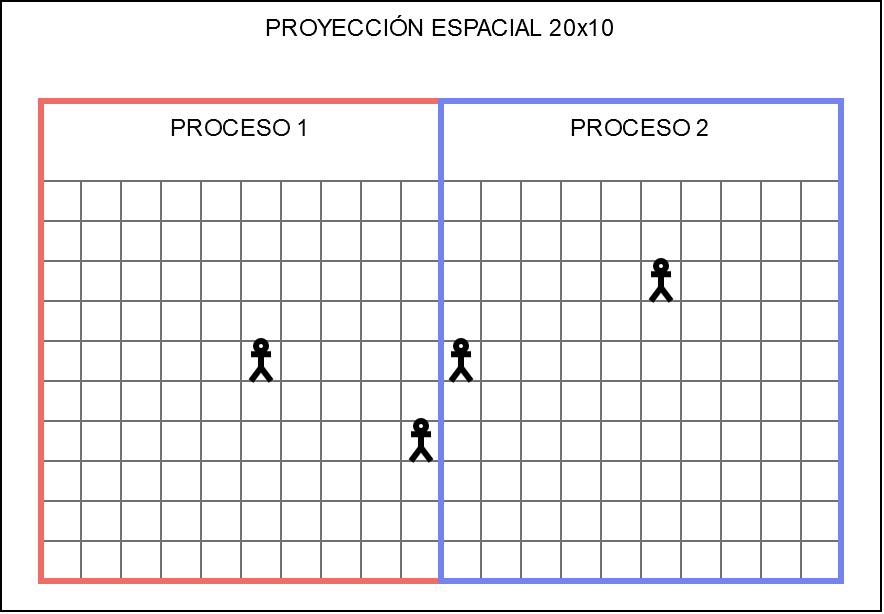
\includegraphics{process_01.png}
	\caption{Partición de una proyeción espacial entre 2 procesos}
\end{figure}

Dado que la principal aplicación de una proyección espacial es obtener
otros agentes que se encuentren en la proximidad, surge un problema:
cuando un agente en el \emph{borde} del proceso solicita los agentes que
lo rodean, recibe solo aquellos que se encuentren en el mismo proceso.

Para solucionar esto, Repast agrega una \emph{zona de amortiguamiento}
como seguridad: cuando un agente se acerca al borde es copiado al
proceso adyacente (como un agente no-local, por lo cual no puede
modificarse, pero permite saber de su existencia). De esta manera,
cuando un agente cercano al borde solicite los agentes que lo rodean,
recibirá correctamente los agentes.

\begin{figure}
	\centering
	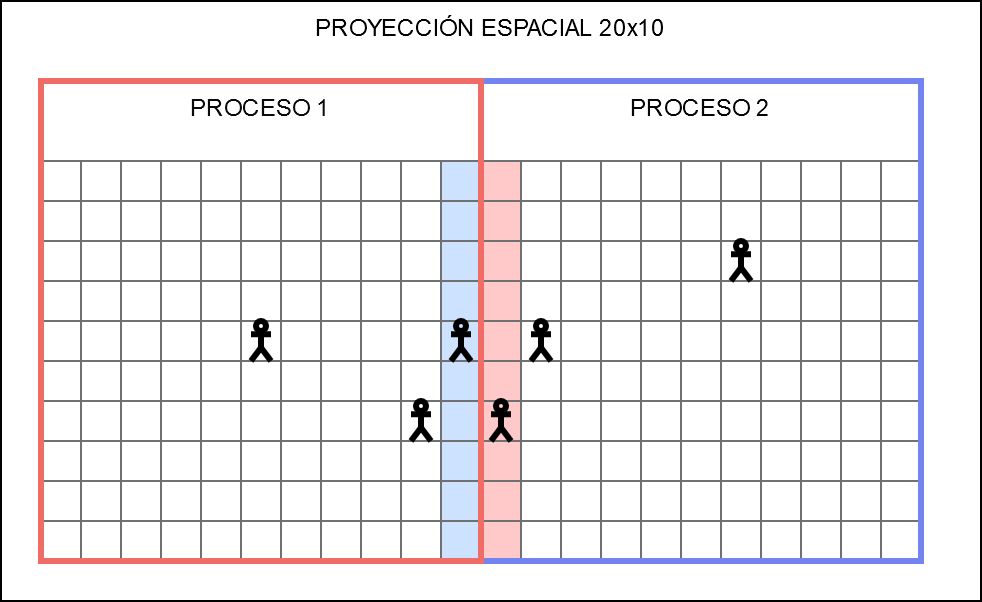
\includegraphics{process_02.png}
	\caption{Partición de una proyección espacial utilizando una zona de amortiguación para copiar agentes}
\end{figure}

En color puede verse toda la información que fue copiada desde el otro
proceso.

El tamaño de la zona de amortiguamiento es definido por el usuario, una
amortiguación chica reduce la comunicación entre procesos pero reduce la
distancia a la cual ven los agentes en otros procesos. Por lo tanto se
debe establecer el mínimo tamaño posible.

	
\section{Simulación de contagio en hospitales}

\subsection{Objetivo}

Dada la complejidad de Repast HPC y el tiempo disponible de la materia
para llevar a cabo el proyecto, se optó por priorizar el paralelismo en
la simulación, realizando mediciones de rendimiento y buscando posibles
mejoras. Por este motivo en la simulación solo se mantuvo una lógica de
transmisión entre los agentes, desplazándose de manera aleatoria sobre
un mapa trivial con paredes en los bordes, solo con el objetivo de
verificar que el modelo funciona correctamente y que los mapas y agentes
son generados de forma correcta (se considera que se brindan las
herramientas necesarias para profundizar en la lógica de la simulación
si se desea).

\subsection{Rendimiento}

Para realizar métricas de rendimiento, se ejecuta reiteradas veces la
simulación combinando distintos parámetros como el tamaño del mapa, la
cantidad de agentes y la distribución del mapa en cantidad de procesos.

De cada combinación realizada se mide el tiempo de ejecución para la
simulación con esas características.

\begin{figure}[H]
	\centering
	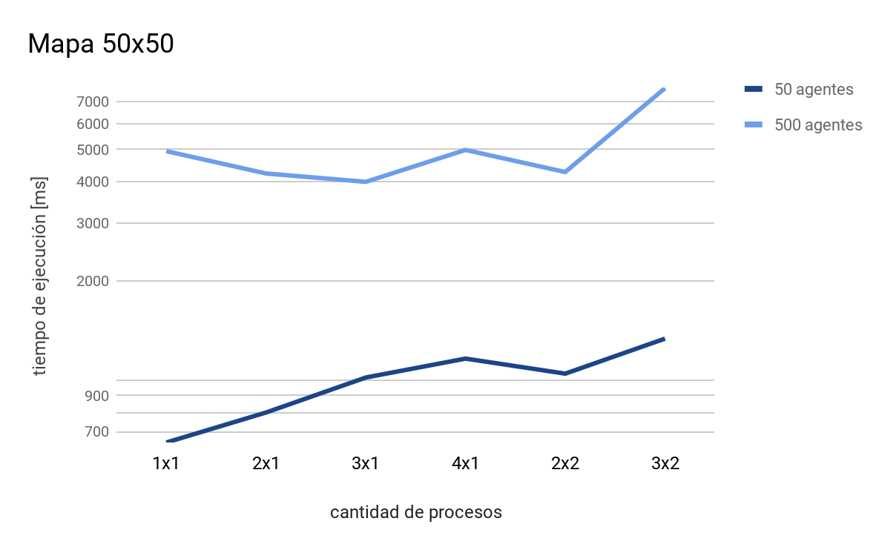
\includegraphics{Rendimiento1.png}
	\caption{Mapa de 50x50 con 50 y 500 Agentes}
\end{figure}

\begin{figure}[H]
	\centering
	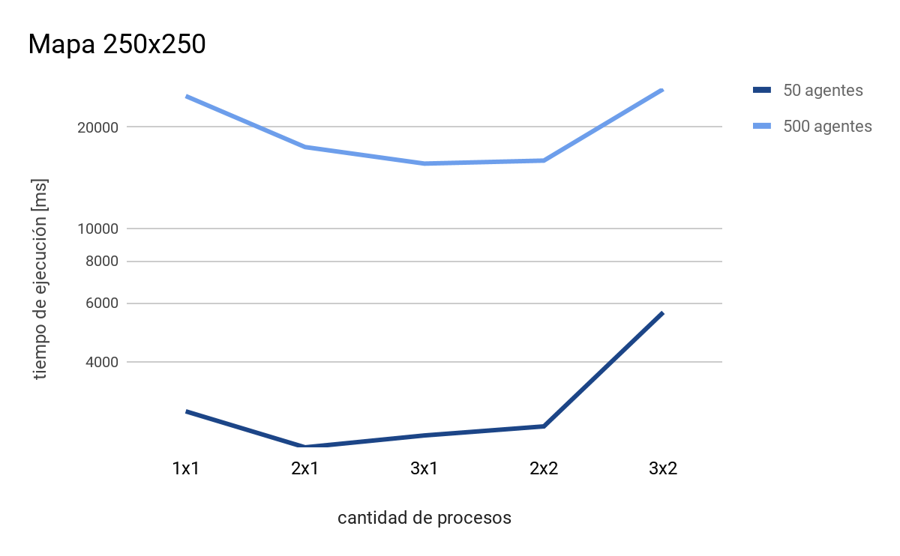
\includegraphics{Rendimiento2.png}
	\caption{Mapa de de 250x250 con 50 y 500 Agentes}
\end{figure}

Como podemos observar, cuando la proyección espacial se trata de un mapa
de tamaño reducido con poca o mediana cantidad de agentes, el
rendimiento no se ve favorecido al aumentar la cantidad de procesos,
sino al contrario, el tiempo de ejecución aumenta, debido al incremento
de comunicación; reduciendo el rendimiento del sistema.

En los siguientes casos, cuando el mapa espacial aumenta a un tamaño de
500x500, sí se puede observar una notable mejora de rendimiento cuando
se ejecuta la simulación en 1 y en 4 procesos, reduciendo el tiempo de
ejecución a aproximadamente la mitad al aumentar el grado de
paralelismo.

\begin{figure}[H]
	\centering
	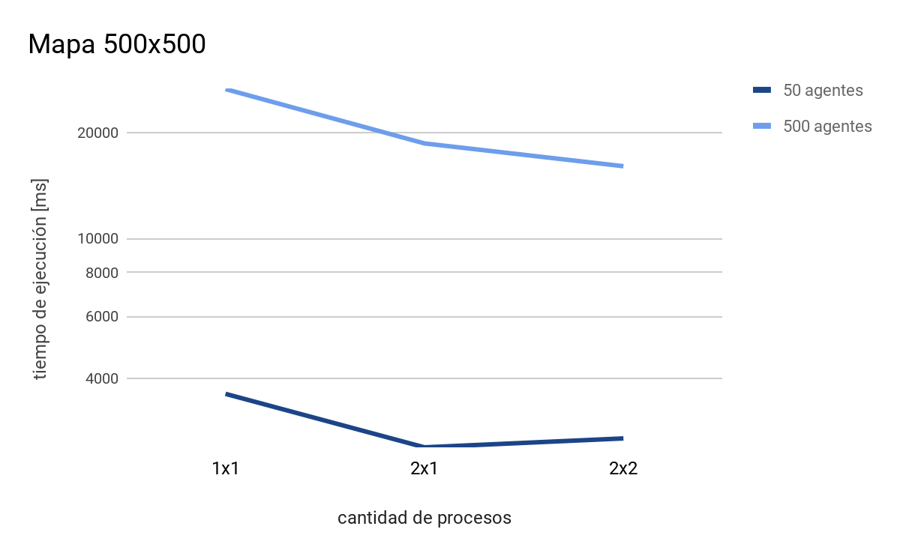
\includegraphics{Rendimiento3.png}
	\caption{Mapa de 500x500 con 50 y 500 agentes}
\end{figure}

\begin{figure}[H]
	\centering
	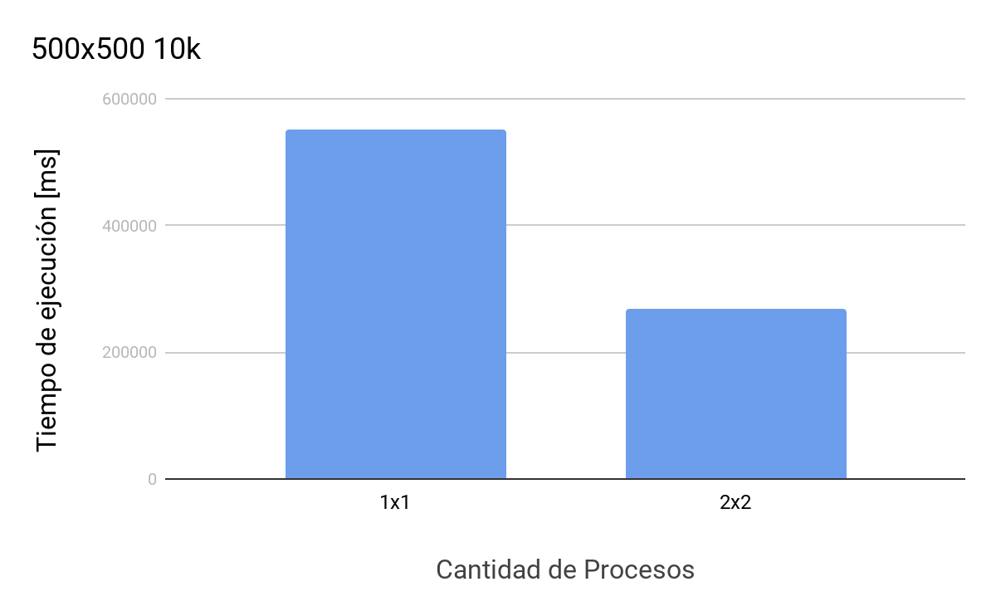
\includegraphics{Rendimiento4.png}
	\caption{Mapa de 500x500 con 10'000 agentes}
\end{figure}

Estos resultados obtenidos se deben a que cuando el nivel de
procesamiento es reducido, la comunicación entre procesos es
excesivamente alta. Por lo que, tratándose de simulaciones que no
demandan un gran procesamiento, no se justifica la paralelización, ya
que el rendimiento no solo no mejorará, sino que se verá afectado, y a
su vez, la complejidad es mucho mayor. Por el contrario, cuando se trata
de simulaciones con una cantidad de agentes mayor, en un espacio
extenso, las mejoras en tiempo de ejecución son muy significativas,
reduciendo el mismo, en algunos casos, a casi el 50\%.

También, es necesario destacar otro factor que influye directamente en
el rendimiento de la simulación que es el balance de procesamiento para
cada proceso. Es decir, si la simulación se ejecuta, por ejemplo, en 4
procesos, el escenario perfecto sería que cada proceso ejecute el 25\%
del procesamiento total. De otra manera, todos los procesos tendrían que
esperarse entre sí, simulando una barrera, hasta que terminen su parte
de la ejecución. Luego, el scheduler puede realizar la sincronización
entre los mismos antes del siguiente tick, y así, que todos comiencen la
ejecución en el mismo instante.

	\section{Conclusión}

Repast for High Performance Computing es un framework muy amplio, de
bajo nivel y que requiere que el modelado se adapte a las
características de la herramienta, debido a su principal objetivo de
maximizar el paralelismo.

Si el objetivo es realizar una simulación sólida, el tiempo de
desarrollo es elevado, debido a los ajustes que se deben realizar al
modelo para adaptarlo a un ambiente paralelo de memoria distribuida
escalable.

En cuanto a lo relacionado al desarrollo, podría modernizarse en ciertos
aspectos, principalmente las dependencias, ya que funciona con una
combinación específica de versiones provista por Repast, algunas del año
2015/16. La información es dispersa y bastante desactualizada, contando
solo con dos commits en 2019.
	
\end{document}